%% ----------------------------------------------------------------
%% Thesis.tex -- MAIN FILE (the one that you compile with LaTeX)
%% ----------------------------------------------------------------

% Set up the document
\documentclass[a4paper, 12pt, oneside]{Thesis}  % Use the "Thesis" style, based on the ECS Thesis style by Steve Gunn
\graphicspath{{figures/}}  % Location of the graphics files (set up for graphics to be in PDF format)

\usepackage{verbatim}  
\usepackage{vector}  
\usepackage{notoccite}
\hypersetup{urlcolor=blue, colorlinks=true}  

\usepackage{silence}
\WarningFilter{sectsty}{Command \underbar has changed.}
\WarningFilter{sectsty}{Command \underline has changed.}
% \usepackage{multirow}
\usepackage{sectsty}
% \usepackage{multirow}
\usepackage{marginnote}
\usepackage{framed}

\chapterfont{\large\centering\bfseries}
\chaptertitlefont{\large\centering\bfseries}
\sectionfont{\normalsize\bfseries}
\subsectionfont{\normalsize\bfseries}
\subsubsectionfont{\normalsize\bfseries}

\hypersetup{pdfborder={0 0 0}, colorlinks=false}  % Black hyperlinks.

\renewcommand{\figurename}{\normalsize Figure}
% Different font in captions
\newcommand{\captionfonts}{\normalsize}
\makeatletter  % Allow the use of @ in command names
\long\def\@makecaption#1#2{%
  \vskip\abovecaptionskip
  \sbox\@tempboxa{{\captionfonts #1: #2}}%
  \ifdim \wd\@tempboxa >\hsize
    {\captionfonts #1: #2\par}
  \else
    \hbox to\hsize{\hfil\box\@tempboxa\hfil}%
  \fi
  \vskip\belowcaptionskip}
\makeatother   % Cancel the effect of \makeatletter


%% ----------------------------------------------------------------
\renewcommand\contentsname{\large{ Table of Contents}}
\renewcommand\listfigurename{\large{List of Figures}}
\renewcommand\listtablename{\large {List of Tables}}
\renewcommand\bibname{References}

\begin{document}

%% ----------------------------------------------------------------

\thispagestyle{empty}
\vspace*{-4cm}

\reversemarginpar
\marginnote{
\begin{framed}
\vspace*{2cm}
\rotatebox{270}{NAME AND SURNAME}
\\[7cm] 
 \rotatebox{270}{M.S. Thesis}
\\[9cm] 
 \rotatebox{270}{2016}
\\[2cm] %
\end{framed}
 }
 
 
\begin{center}
\vspace*{5cm}
\large{THESIS TITLE} 
\\[8cm] %
\large{NAME AND SURNAME} 
\\[10cm] %
I\c{S}IK UNIVERSITY
\\
2016
\\[2cm] %
\end{center}
 
\clearpage

%% ----------------------------------------------------------------

\thispagestyle{empty}
\begin{center}
\vspace*{1cm}
\large{THESIS TITLE} 
\\[6cm] 
\large{NAME AND SURNAME} \\
\normalsize {
B.S., Computer Engineering, I\c{S}IK UNIVERSITY, 2009 \\
B.S., Mathematics Engineering, I\c{S}IK UNIVERSITY, 2009 \\[5cm]%
Submitted to the Graduate School of Science and Engineering \\
in partial fulfillment of the requirements for the degree of \\
Master of Science\\
in\\
Computer Engineering \\[3cm] 
I\c{S}IK UNIVERSITY \\
2016 }
\end{center}

\frontmatter     

%% ----------------------------------------------------------------

\thispagestyle{empty}
\begin{center}
\vspace*{-0.9cm}
I\c{S}IK UNIVERSITY \\ 
GRADUATE SCHOOL OF SCIENCE AND ENGINEERING \\[4cm]
THESIS TITLE\\[3cm]
NAME AND SURNAME\\[3cm]
\end{center} 
\begin{flushleft}
APPROVED BY:\\[1.5cm]

Assoc. Prof. Name Surname \hspace{0.85cm} I\c{s}{\i}k University
\hspace{1cm}\rule[0em]{8em}{0.5pt}\\[0.2cm](Thesis Supervisor)\\[1.2cm]

Prof. \hspace{2.9cm}I\c{s}{\i}k
University\hspace{1.1cm}\rule[0em]{8em}{0.5pt}\\[2cm]

Assist. Prof. \hspace{1.8cm} I\c{s}{\i}k University 
\hspace{0.9cm}\rule[0em]{8em}{0.5pt}\\[3cm]

APPROVAL DATE:
\hspace{2.2cm} ..../..../....
\end{flushleft}
\setmarginsrb           {4cm}  % left margin
                        {2.5cm}  % top margin
                        {2.5cm}  % right margin
                        {2.5cm}  % bottom margin
                        {0cm}  % head height
                        {0cm}  % head sep
                        {0cm}  % foot height
                        {1.3cm}  % foot sep

\clearpage

%% ----------------------------------------------------------------

\addtotoc{Abstract}  
\abstract{ 
\noindent The rapid advancement of generative models has
significantly increased the realism of synthetic audio and video,
commonly referred to as deepfakes. This paper reviews key
approaches in deepfake detection, including visual artifact detec
tion, temporal inconsistency modeling, and multi-modal analysis.
Wecompare these methods, analyze their limitations, and identify
open challenges. Finally, we position our research direction
within this evolving landscape, focusing on robust, real-time, and
generalizable detection systems. 

\vspace{1em}

\noindent In this study, we present a correlation based transition model and a proposal function that incorporate partition dependency in particle filtering in a computationally tractable manner. We test our algorithm on challenging examples of occlusion, clutter and drastic changes in relative speeds of partitions. Our successful results with as low as 10 particles per partition indicate that the proposed algorithm is both robust and efficient.

\vspace{1em}

\noindent \textbf {\small{Keywords: Model-based vision, generic wireframe}}
}

%% ----------------------------------------------------------------

\clearpage \addtotoc{\"{O}zet} %%
\ozet { 
\noindent 
\vspace{1em}
\noindent 
\vspace{1em}
\noindent \textbf {\small{ Anahtar kelimeler: }}
}

\clearpage  

%% ----------------------------------------------------------------

% Acknowledgements page
\acknowledgements{
\addtocontents{toc}{\vspace{1em}}  
\noindent This study was supported by The Scientific and
Technological Research Council of Turkey (T\"{U}B\.{I}TAK) Grant No: 
}
\clearpage  

%% ----------------------------------------------------------------

% Dedicated to
\pagestyle{empty}  
\dedicatory{To\ldots}

%% ----------------------------------------------------------------

\addtocontents{toc}{\protect\thispagestyle{empty}}
\tableofcontents  % Write out the Table of Contents

%% ----------------------------------------------------------------

\listoftables  % Write out the List of Tables

%% ----------------------------------------------------------------

\listoffigures  % Write out the List of Figures

%% ----------------------------------------------------------------

\setstretch{1.5}  
\clearpage  % Start a new page
\listofsymbols{ll}  % Include a list of Abbreviations (a table of two columns)
{
\textbf{2-D} & \textbf{2} \textbf{D}imension \\
\textbf{3-D} & \textbf{3} \textbf{D}imension \\
\textbf{PF} & \textbf{P}article \textbf{F}iltering}

%% ----------------------------------------------------------------

\mainmatter   
\pagestyle{plain}
\chapter{Introduction} 
Stochastic approach to tracking is driven by a state--space model of the tracking object. The state of the object is estimated with a probability density function, which was for convenience assumed to be Gaussian in earlier works. Kalman filter \cite{kalman1960}, the most popular tracking algorithm with Gaussian probability density assumption, is a provably optimal estimator for linear systems. However, Kalman filter fails in cluttered scenes, occlusions, and sudden changes of state, for which the probability density of state is multimodal. 

This thesis is organized as follows. In Chapter \ref{ch:literature_survey} we will introduce the original condensation algorithm and its extension with PFFL. We will detail our approach in Chapter \ref{ch:approach}, including the observation model, transition model and the proposal function. We will present our experimental results in Section \ref{ch:results} and conclude our work in Section \ref{ch:conclusion}.

\chapter{Literature Survey} 
\label{ch:literature_survey}
\section{Particle Filtering}
\label{sec:particle_filtering}
We aim to track regions chosen on an object in a sequence of image frames. The states of these regions will be represented by \textit{partitions} where the current state of partition $i$ is denoted by $x_i$. In our implementation each partition has a reference image (template) and a state that consists of the partition's coordinates in the 2D image frame. 

When we model state transition as a Markov chain with independent observations, the posterior probability of state for a particle is defined as:
\begin{equation}
\label{eq:posterior_prob_1}
p(x_i^t|\mathbf{Z}^t) \propto p(\mathbf{z}^t|x_i^t)p(x_i^t|\mathbf{Z}^{t-1})
\end{equation}

\begin{equation}
\label{eq:posterior_prob_2}
p(x_i^t|\mathbf{Z}^{t-1}) = \sum_{x_i^{t-1}} p(x_i^t|x_i^{t-1})p(x_i^{t-1}|\mathbf{Z}^{t-1})
\end{equation} 

Probability of the assumed state (\ref{eq:posterior_prob_1}) $x_i^t$ is proportional to the probability of reaching this state after observations $\mathbf{Z^{t-1}}=\{\mathbf{z}^{0},\cdots,\mathbf{z}^{t-1}\}$ and the probability of the current observation in this state. Probability of transition from the previous probability density to the assumed state (\ref{eq:posterior_prob_2}) is found over the dynamic transition model and the posterior probabilities of this partition's particles from the previous time step. Reader is referred to \cite{Isard98condensation} for a complete derivation of posterior probability of state. 

\subsection{Condensation algorithm}
\label{sec:condensation}
Condensation algorithm \cite{Isard98condensation} extends posterior probability density approximation to a sequence of frames. The iteration capitalizes on Markov chain assumption, i.e. the likelihood of a state depends on the probability density of the previous state, the probability of transition into the current state using the dynamic model and the current observation. 

Given the posterior probability density for the previous time step $p(x_i^{t-1}|\mathbf{Z}^{t-1})$, which is represented with a set of particles and their probabilities $\{s_{ik}^{t-1},\pi_{ik}^{t-1}\}$, $k=\{1,\cdots,M\}$, condensation algorithm proceeds as follows:

\begin{enumerate}
\item Sample $M$ particles from $\{s_{ik}^{t-1},\pi_{ik}^{t-1}\}$.
\item Predict new states for particles using the dynamic model $s_{ik}^t=p(x_i^t|x_i^{t-1}=s_{ik}^{t-1})$.
\item Evaluate particles with respect to the current observation $\pi_{ik}^t\propto p(\mathbf{z}^t|x_i^t=s_{ik}^t)$.
\end{enumerate}

The dynamic model in this algorithm consists of drift and diffusion. Drift is deterministic motion defined with velocity and acceleration, and is common for all particles of a partition. Diffusion on the other hand is Brownian motion; random movements that split particles at the identical state and enable search in the image space through random walk. 

\chapter{Approach} 
\label{ch:approach}
The PFFL algorithm leverages the dependent behavior of multiple partitions on a single object. In the general sense, the interdependency of partitions can be incorporated either as constraints in the dynamic model $p(x_i^t|x_i^{t-1})$, or in choosing $N$ particles from the posterior of $N$ partitions through proposal function $g(\mathbf{x}^t)$. In this study we first propose a transition model that provides an estimation for dependent drift of partitions. Second, we relieve the factorization constraint in the proposal function $g(\mathbf{x}^t)$ and propose a simple and computationally efficient model for modeling the joint probabilities of partitions.

\chapter{Results and Discussion} 
\label{ch:results}
Figure (\ref{fig:proposal_function}) presents a 2D plot of the magnitude of the proposal function for the partition at the mouth of a gourami. When the scaling factor $\sigma_p$ is low, relative motion between the partitions are more restricted and the object is considered to be more rigid. The partitions move more freely against each other as the scaling factor increases. 

\begin{figure}
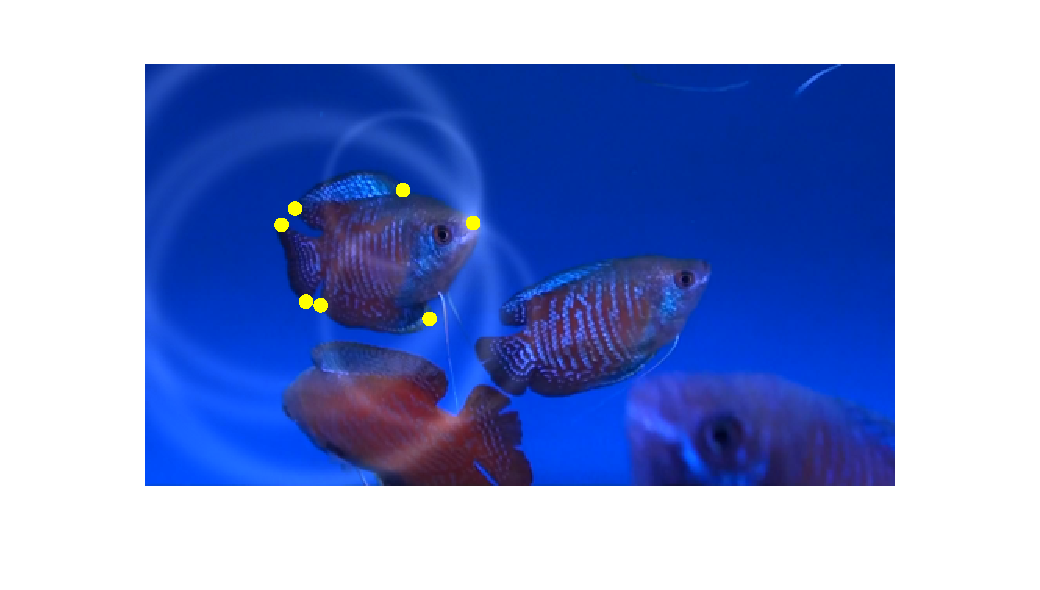
\includegraphics[width=1\textwidth,height=0.44\textheight]{proposal_function.eps}
\includegraphics[width=1\textwidth,height=0.44\textheight]{probability_field.eps}
\caption{Probability field for the partition at the mouth of a gourami. Top: The magnitude of the proposal function is depicted with shades of gray. For demonstration purposes, the scaling factor is chosen higher than the actual implementation. Bottom: 3D plot of the probability field.}
\label{fig:proposal_function}       
\end{figure}

In the first two tracking scenarios we test the capabilities of these three algorithms (the proposed algorithm, PFFL and SPOT) to deal with occlusion and clutter. In both scenarios the task is to track an object in a crowded scene of similar objects. As shown in Table (\ref{table:videos}), \textit{platty} is a publicly available high-definition video of a crowded school of fish. \textit{Skydiving} is a challenging video as it is low resolution and the skydivers' jumpsuits are very similar. In the third scenario we assess the tracking algorithms on sudden changes in transition dependencies of partitions. In this scenario we use a face video from the MMI facial expression database \cite{pantic2005}. This video is carefully selected to exhibit relative motion and speed reversals (e.g. blinking, neutral-smile-neutral) together with rigid body motion (e.g. head movements) of the features. 

\begin{table}
\centering
\begin{tabular}{|l|l|l|}
	\hline
		Video & Resolution & Frames \\
	\hline	
		Platty \cite{fishcouk} & 1080$\times$1920& 110\\
	\hline
		Skydiving \cite{zhang2013} & 480$\times$656& 300\\
	\hline
		Face \cite{pantic2005} & 576$\times$720& 127\\
	\hline
\end{tabular}
\caption{Evaluation of tracking algorithms on three scenarios; platty, skydiving and face. The length of segment that is used in experiments is indicated by the number of frames.}
\label{table:videos}
\end{table}

Figure (\ref{fig:error_platty_comparison}) compares tracking performances of the proposed algorithm, PFFL and SPOT. In this figure, average relative error over 12 tracking points is plotted against the frame numbers. Tracking error in PFFL parts from the other two algorithms starting from frame 20. At the end of the experiment, average relative error with PFFL is about an order of magnitude higher than the other two algorithms. SPOT occasionally drifts due to the imprecision of its observation model. Both proposed algorithm and SPOT highly benefit from the configuration based proposal function and manage to keep the general structure of platty until the end of the experiment. 

\begin{figure}
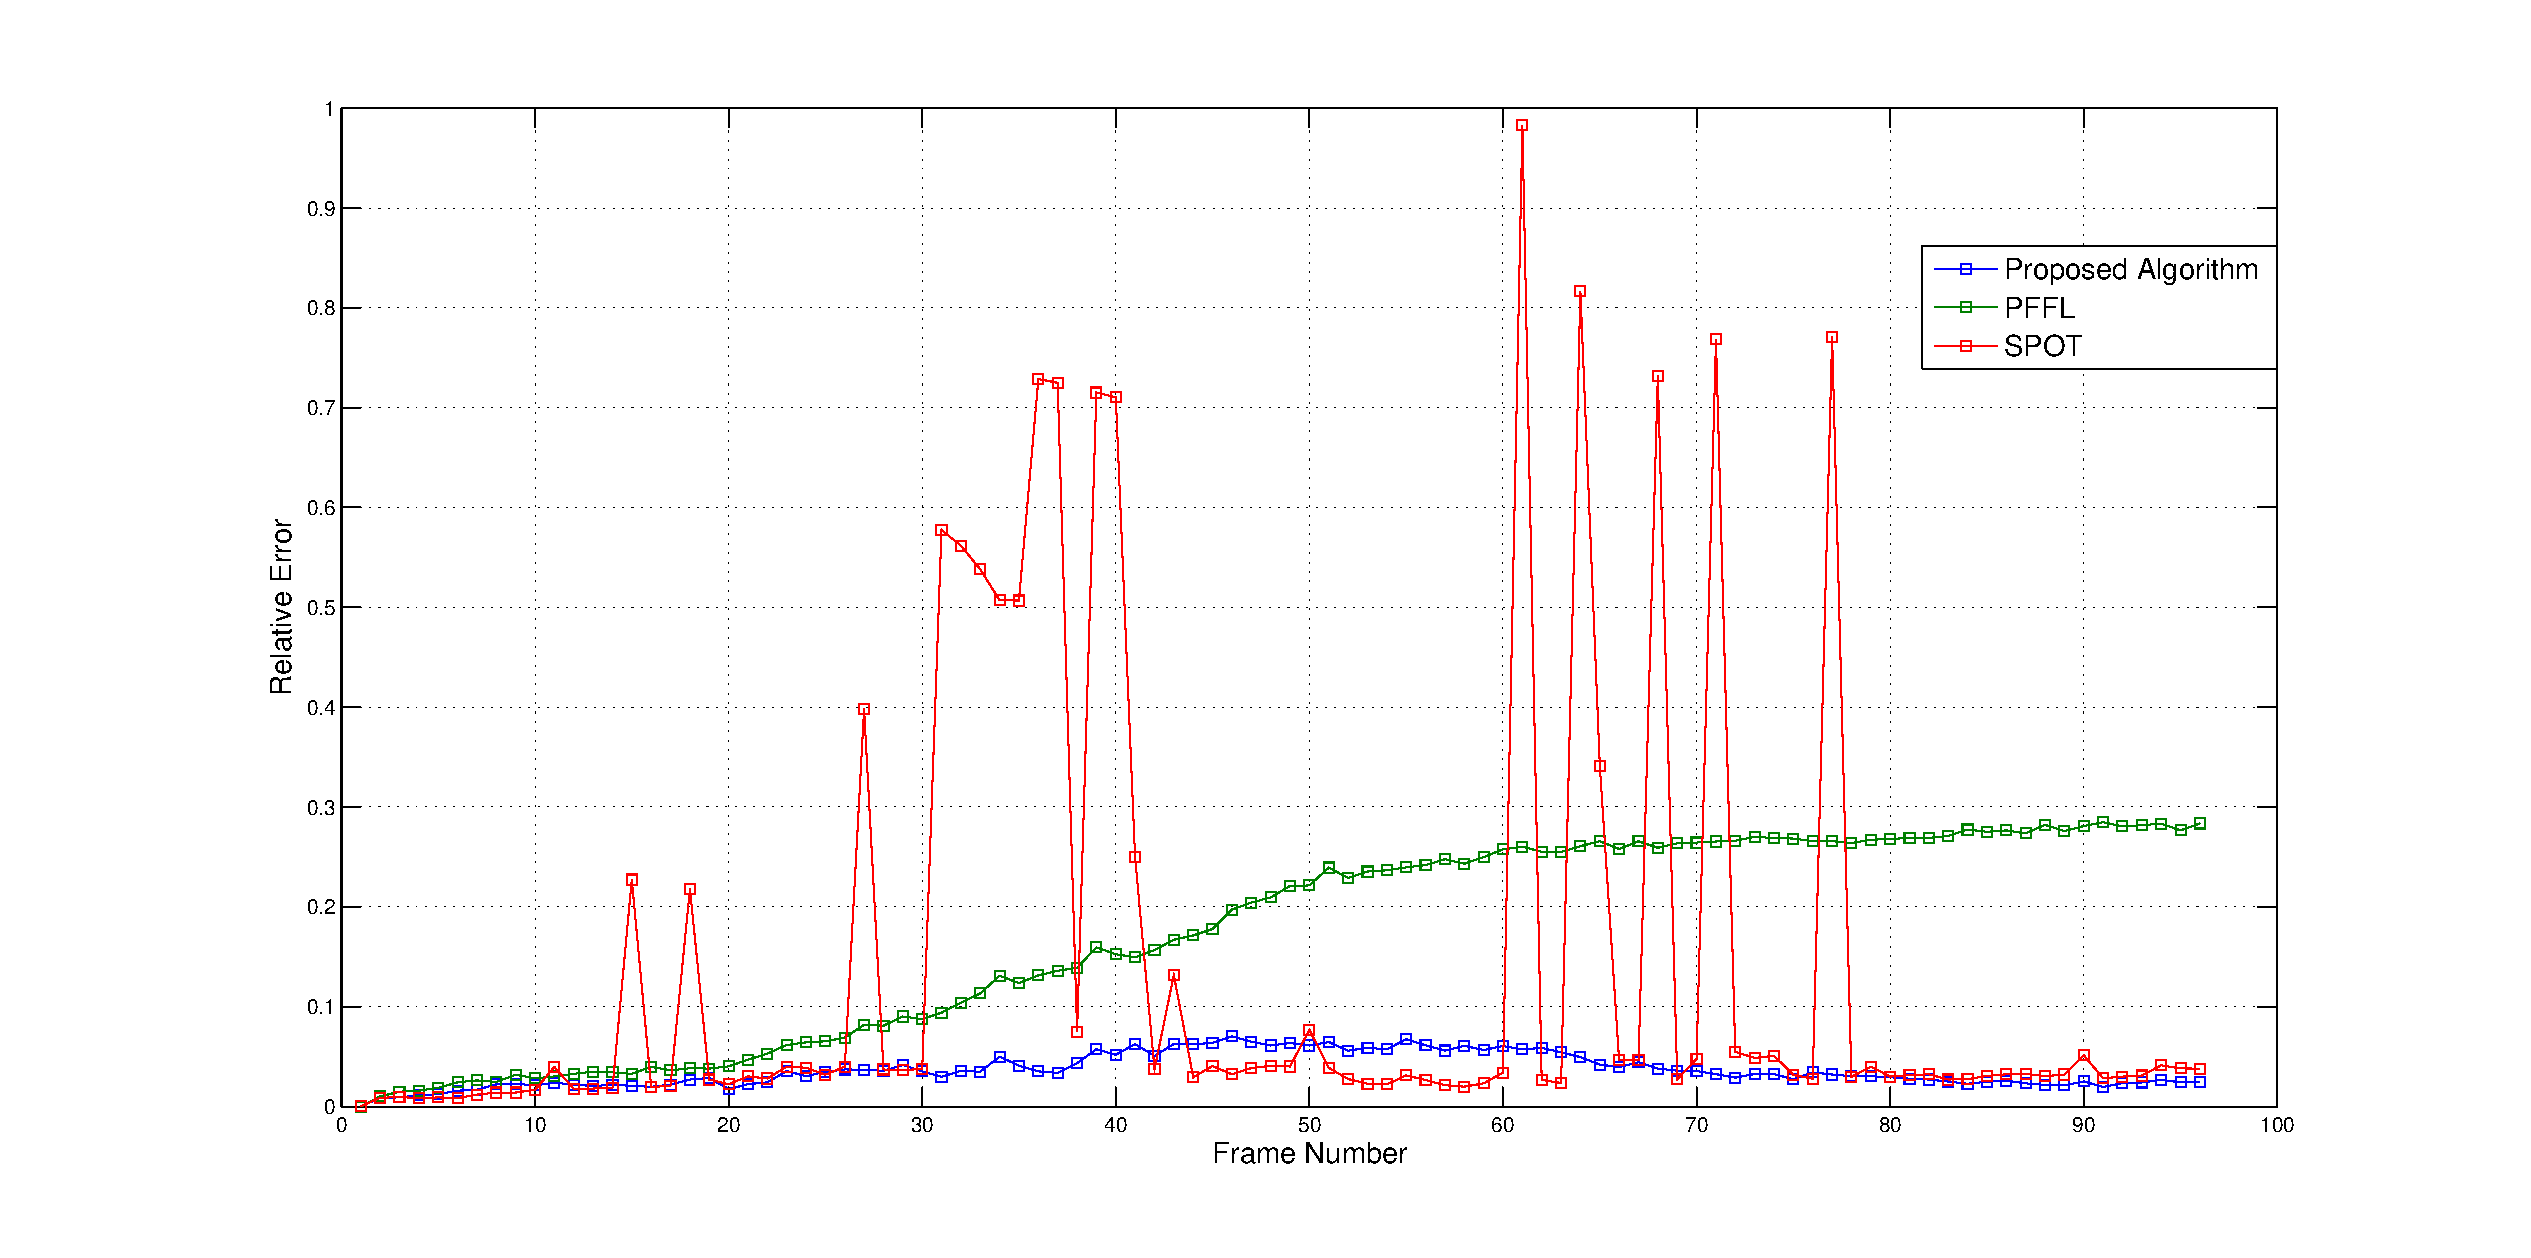
\includegraphics[width=1\textwidth]{error_platty_comparison.eps}
\caption{Comparison of average error on platty for the proposed algorithm (10 particles), PFFL (50 particles) and SPOT. Data markers depict the average relative error for 12 partitions for each frame.}
\label{fig:error_platty_comparison} 
\end{figure}

\chapter{Conclusion} 
\label{ch:conclusion}
In this paper we present two contributions to tracking multiple partitions of a deformable object with particle filtering. Our first contribution is in \textit{drift}; the deterministic motion of a partition with respect to other partitions. The second contribution is in selection of particles from probability densities of partitions such that the set of particles represent a viable and likely current state of the object. 

%% ----------------------------------------------------------------

\clearpage 
\addtotoc{Reference}
\bibliographystyle{IEEEtran}
\bibliography{bibliography}

\end{document}  

%% ----------------------------------------------------------------